\documentclass[11pt,a4paper]{article}

\usepackage[margin=2.3cm]{geometry}
\usepackage[T1]{fontenc}
\usepackage{graphicx}
\usepackage{amsmath}
\usepackage{booktabs}
\usepackage{array}
\usepackage{tikz}
\usetikzlibrary{arrows.meta,positioning}
\usepackage{caption}
\usepackage{float}
\usepackage[section]{placeins}
\usepackage[colorlinks=true,linkcolor=blue!50!black,urlcolor=blue!50!black]{hyperref}

\captionsetup{font=small,labelfont=bf}
\Urlmuskip=0mu plus 1mu
\def\UrlBreaks{\do\/\do\-\do\?\do\=\do\_\do\.}
\setlength{\parindent}{0pt}
\emergencystretch=2em
\setlength{\parskip}{0.45em}
\renewcommand{\arraystretch}{1.08}

\newcommand{\auc}{AUC-ROC}
\newcommand{\trp}{\texttt{topic\_rate\_prior}}
\newcommand{\weightsurl}{https://drive.google.com/drive/folders/1IQb9xincr7PjG4kQvqEmj8jBBezRqQRZ?usp=drive_link}

% A figure that is skipped (with a grey placeholder) when the image file is missing, so the report always compiles.
\newcommand{\maybefig}[2]{\IfFileExists{#2}{\includegraphics[#1]{#2}}{\fbox{\parbox{0.7\linewidth}{\centering\small\vspace{1.2cm}Image \texttt{\detokenize{#2}} not found\vspace{1.2cm}}}}}

\title{\textbf{SpillThePaper}\\[2pt]
\large From Past Papers to a Predicted, Solved and Personalised Exam\\[2pt]
\normalsize Final Report, AI Course Project, Track A (Application Development)}
\author{Minahil Basalat (24L-3082) \and Iman Abid (24L-0707) \and Khadija Rao (24L-3042)\\[3pt]
FAST-NUCES}
\date{}

\begin{document}
\maketitle

\begin{abstract}
Students at FAST-NUCES can find hundreds of past quizzes, mid-terms and finals, but deciding what to study from them is
manual guesswork. SpillThePaper turns this archive into evidence-based exam preparation. The system collects and
cleans 3{,}567 files from a public student archive, recovers scanned papers with OCR, splits papers into 10{,}538 questions
with marks, type and difficulty estimates, and discovers per-subject topics. Because the archive has no labels, we define a
supervised task: given a subject, a topic and a target exam, predict whether the topic appears, using only earlier papers.
On a leakage-safe, time-split dataset of 3{,}465 rows (37 subjects) a logistic regression, a random forest and a PyTorch
multi-layer perceptron reach a test AUC-ROC of 0.850, 0.871 and 0.857, against 0.824 to 0.836 for simple history rules.
The learned models rank slightly better and are clearly more precise than the rule ``appeared at least five times''
(precision 0.58 to 0.67 against 0.46), but the confidence intervals still overlap with the best rule, so we do not claim
a statistically separated gain. On top of the models we built a Streamlit application: a past-paper browser, a predicted-paper
generator with a realistic structure, difficulty mix and timer, archived and AI-written solutions, PDF export, photo-based
grading of a student's own answers, weak-area analysis and a personalised follow-up paper. Optional language-model steps rewrite
questions and write missing solutions in the background, with real, tidied past questions as the fallback. Every number in this
report comes from a run of the code in the repository (\url{https://github.com/Minahilbasalat/SpillThePaper}).
\end{abstract}

\tableofcontents
\newpage

%=====================================================================
\section{Introduction}
\label{sec:intro}

Students at FAST-NUCES often have access to many past quizzes, mid-terms and finals, but the collection is large,
unstructured and inconsistent. SpillThePaper aims to turn this archive into evidence-based exam preparation. It estimates
which syllabus areas are likely to appear in an upcoming exam, generates a tentative paper with a realistic structure,
shows solutions, times the student, and then analyses the student's own answers to personalise the next practice paper.
It is a study aid and does not guarantee what will appear in a real exam.

The project was delivered in phases. Phase~1--2 defined the problem and built the data foundation; Phases~3--4 designed,
trained and evaluated the topic-appearance models; Phase~5 built the application; Phase~6 (this report) merges all of it.
Table~\ref{tab:phases} maps the phases to sections.

\begin{table}[!htb]
\centering
\small
\begin{tabular}{p{4.6cm}p{10.4cm}}
\toprule
Phase & Content and section \\
\midrule
1--2: Problem and data & Problem statement, audience, AI justification (Section~\ref{sec:problem}); collection, cleaning, features, EDA (Section~\ref{sec:data}); data repair, OCR and question bank (Section~\ref{sec:repair}) \\
3: Model architecture & Task definition, topic discovery, features, models, MLP, loss, optimiser, tuning (Sections~\ref{sec:task}, \ref{sec:models}) \\
4: Training and evaluation & Validation strategy, metrics, results, error analysis, bias check (Section~\ref{sec:eval}) \\
5: Application & Backend, language-model layer, grading and personalisation, user interface (Sections~\ref{sec:backend}--\ref{sec:ui}) \\
6: Documentation & Testing, limitations, future work, reproducibility (Sections~\ref{sec:testing}--\ref{sec:repro}) \\
\bottomrule
\end{tabular}
\caption{Phases of the project and where this report covers them.}
\label{tab:phases}
\end{table}

%=====================================================================
\section{Problem Definition}
\label{sec:problem}

\subsection{Problem statement}
University students often have access to a large collection of past quizzes, mids and finals, but deciding what to study
from them is difficult. Papers span many semesters and courses, and students usually review them by hand and rely on
guesswork, senior advice or assumptions about what might appear again. This creates several problems:
\begin{itemize}
\item \textbf{Patterns are hard to see.} Recurring topics, question types, difficulty and mark distributions are easy to miss
when reading many papers manually.
\item \textbf{Syllabi change.} A topic frequent in old papers may have been removed or changed.
\item \textbf{Too many papers, too little time.} Nobody can study all of them.
\item \textbf{Over-preparing predicted topics.} Studying only frequent topics leaves students unprepared for surprises.
\item \textbf{Preparation is not personal.} Past-paper practice does not tell a student which of \emph{their} areas is weak.
\item \textbf{Time management is overlooked.} Students rarely test their speed under a realistic exam duration.
\end{itemize}

\subsection{Target audience}
The primary users are FAST-NUCES undergraduates (starting with CS, AI and SE courses) preparing for quizzes, mids and
finals. Supported courses are those with enough history to find patterns; courses with very few papers are flagged as
low-confidence and receive no prediction. Students who add their own papers or course outline are a secondary audience.
Students outside this exam culture and courses with no history are not targeted.

\subsection{AI justification}
\label{sec:ai}
A rule such as ``if a topic appeared five times, predict it'' is easy to implement but insufficient, because:
(i) the input is unstructured text in which the same concept is worded differently, so NLP is needed to find topics and
question types; (ii) frequency, recency, assessment type, marks, difficulty and syllabus relevance interact;
(iii) exam patterns drift over time; (iv) predictions are uncertain, so the system should estimate a likelihood and keep
less-predictable areas in the paper; (v) matching old questions to a current syllabus needs similarity of meaning rather
than exact keywords; and (vi) personalisation means learning from a student's performance. Section~\ref{sec:eval} tests the
first claim honestly: the rule baselines turn out to be strong, and the learned models' advantage is moderate.

%=====================================================================
\section{Data Foundation}
\label{sec:data}

\subsection{Data source and collection}
The data come from the public GitHub repository \emph{Academic-Time-Machine}, a student-maintained archive of past papers,
outlines, books and notes~\cite{atm} (8{,}562 files at the pinned commit \texttt{e0e1975}). The structure is irregular: subject folders
contain assessment folders, term folders or loose files; term and year appear in folder names, file names, ranges or not at
all. Three configurable scripts discover the file tree, filter it, and download the selected files with a SHA-256 manifest.
Subject names are never hard-coded; rules live in configuration files. Table~\ref{tab:collection} summarises the result.
All 3{,}567 selected files were downloaded without failure. The raw files are not redistributed.

\begin{table}[!htb]
\centering
\small
\begin{tabular}{lr}
\toprule
Item & Files \\
\midrule
Files in the repository & 8{,}562 \\
Selected exam material & 3{,}567 \\
\quad quizzes / mids / finals / outlines / unspecified & 1{,}400 / 1{,}215 / 819 / 124 / 9 \\
\quad by format: PDF / Word / photograph & 2{,}911 / 312 / 344 \\
Excluded (code, slides, notes, assignments, non-exam folders) & 4{,}995 \\
\bottomrule
\end{tabular}
\caption{Results of filtering the repository.}
\label{tab:collection}
\end{table}

No reliable instructor information exists in the file paths, so no professor-specific analysis is attempted.

\subsection{Preprocessing}
Text is extracted with PyMuPDF~\cite{pymupdf} (it kept words correctly spaced where another reader merged them) and \texttt{python-docx}.
PDFs with almost no text, and photographs, are flagged for OCR (Section~\ref{sec:ocr}). The 3{,}567 files become 3{,}443
exam papers and 124 course outlines, with raw columns (subject, assessment type and number, term, year), extracted columns
(total marks, question count, pages, words, year from the header) and derived flags (solution, merged compilation, retake, lab).
Reading the paper header recovered the year of 666 papers that the path did not describe.

\textbf{Missing values} are never a reason to delete a row: values are recovered from a second source where possible,
impossible values are treated as missing, and a paper without text is excluded from text analysis only. \textbf{Duplicates}
are removed in four ordered steps (Table~\ref{tab:funnel}). \textbf{Outliers} are flagged, not removed, using the 1.5-IQR rule
per assessment type on numeric columns only (257 of the clean papers flagged on at least one column). \textbf{Features}
follow Table~\ref{tab:featstrat}: one-hot for low-cardinality categories, $\log(1+x)$ and z-score scaling for skewed counts, and
min--max scaling for year. Scaling parameters used by models are learned on the training split only.

\begin{table}[!htb]
\centering
\small
\begin{tabular}{lrr}
\toprule
Cleaning step & Excluded & Remaining \\
\midrule
Start & -- & 3{,}443 \\
Exact duplicates (same SHA-256) & 160 & 3{,}283 \\
Same-text duplicates & 50 & 3{,}233 \\
Merged compilations (``all finals merged'') & 51 & 3{,}182 \\
Solution companions (paper also exists without solution) & 309 & 2{,}873 \\
\bottomrule
\end{tabular}
\caption{Papers remaining after each cleaning step.}
\label{tab:funnel}
\end{table}

\begin{table}[!htb]
\centering
\small
\begin{tabular}{p{4.2cm}p{10.8cm}}
\toprule
Feature group & Treatment and reason \\
\midrule
Assessment type, term & One-hot (few categories, no order); ``Unknown'' kept as its own category \\
Subject & Not one-hot (131 values, many rare); kept for grouping, with a paper-count feature \\
Flags (solution, retake, lab, has text) & Binary 0/1 \\
Year & Min--max scaled; unknown years stay missing with a flag \\
Pages, words, marks, question count & $\log(1+x)$ then z-score (skewness 1.0 to 4.5); missing values median-filled by type with a flag \\
Paper text & Vectorised later (TF-IDF); no numeric scaling \\
\bottomrule
\end{tabular}
\caption{Feature strategy of the data foundation.}
\label{tab:featstrat}
\end{table}

\subsection{Exploratory data analysis}
\label{sec:eda}
Figures~\ref{fig:eda1} and~\ref{fig:eda2} show the initial snapshot of the data (before OCR). Quizzes are the largest group
(1{,}400 files), followed by mids and finals. Coverage is uneven: a few subjects have many papers, most have few, and the
recent years are thinner than the middle ones. About a third of the files had no extractable text, and finals and mids were
affected much more than quizzes: this motivated the OCR step.

\begin{figure}[!htb]
\centering
\maybefig{width=0.48\linewidth}{figures/01_papers_by_type.png}\hfill
\maybefig{width=0.48\linewidth}{figures/03_papers_by_year.png}
\caption{Papers by assessment type (left) and by year (right) in the initial snapshot.}
\label{fig:eda1}
\end{figure}

\begin{figure}[!htb]
\centering
\maybefig{width=0.78\linewidth}{figures/04_subject_year_heatmap.png}\\[4pt]
\maybefig{width=0.5\linewidth}{figures/06_text_coverage.png}
\caption{Papers per subject and year (top) and share of papers with readable text by assessment type before OCR (bottom).}
\label{fig:eda2}
\end{figure}

%=====================================================================
\section{Data Repair, OCR and the Question Bank}
\label{sec:repair}

After the first models were trained, an audit of the data, the tables and the code found problems that limited both the
models and the application. This section describes what was found and how it was fixed. All later results use the
repaired data.

\subsection{Audit findings}
\begin{itemize}
\item About a third of the clean papers had no text because they are scans, and the newest years were hit hardest.
\item About 31\% of ``questions'' came from files flagged as solutions, so answer text was mixed into the question bank.
\item Questions carried no marks, type, difficulty or linked solution.
\item Exam rules, page headers and OCR garbage had become fake questions and fake topics.
\item Duplicate subject names (PDC and Parallel and Distributed Computing, SPM and Software Process Management and Metrics,
DW and Data Warehousing and Data Mining) split one course's history.
\item Only a small share of questions (about 4\% on the data audited) has a near-duplicate among earlier questions of the same
subject. A predicted paper therefore cannot be built by re-serving old questions.
\end{itemize}

\subsection{OCR recovery of scanned papers}
\label{sec:ocr}
A Tesseract-based module~\cite{tesseract} renders PDF pages at about 216~dpi, corrects phone-photo rotation (EXIF first, then orientation
detection), rebuilds text line by line so the question segmenter still works, and returns a confidence per file. A file is
accepted only with at least 30 words and a mean confidence of at least 55. Tests on synthetic scans exposed a real bug:
Tesseract's automatic page mode returns nothing on sparse pages, which an automatic fallback to single-block mode fixed.
Of the 1{,}123 flagged files, 742 were accepted (median 400 words, median confidence 82.2), 379 were rejected as low quality
(mostly handwritten answer sheets and poor photographs) and 2 failed (Figure~\ref{fig:ocr}). Subjects with no readable paper
fell from 24 to 0, and papers without readable text fell from about a third to 11.1\%.

\begin{figure}[!htb]
\centering
\maybefig{width=0.85\linewidth}{figures/fig_ocr_extraction.png}
\caption{Text extraction method of the 3{,}567 files (left) and the OCR outcome of the 1{,}123 flagged scans (right).}
\label{fig:ocr}
\end{figure}

\subsection{Question segmentation and cleaning}
A rule-based segmenter splits each readable paper into questions with three strategies in order: explicit markers
(\texttt{Question 1}, \texttt{Q2}), numbered items, and a paragraph fallback. Worked solutions, grading tables and headers are
removed. Cleaning then removed exam-conduct text and page furniture (``National University of Computer and Emerging
Sciences, Lahore Campus | Page 3 of 7''): a chunk is dropped only if it has exam-rule cues and no task signal, so real
questions that merely mention ``question paper'' are kept. This dropped 264 chunks, 103 of them from Computer Networks Lab,
whose apparent topic quality (silhouette 0.449) was an artefact of near-copies; after cleaning it fell to a normal 0.105.
A regular expression that froze on very long text was found and replaced with a safe one, guarded by a test. A word-based
quality score separates OCR garbage (about 0.29) from real questions (median 0.99); garbled questions are flagged, never
used to build papers, and listed with a warning. The final question bank has 10{,}538 questions (7{,}780 before OCR).

\subsection{Question-level features}
A rule-based module extracts, for every question: marks (parsed for about half of the questions), the answer text where
the paper includes one, a question type, a Bloom level of the task verb, and a difficulty proxy. Difficulty is explicitly a
proxy: Bloom level, length and share of marks, bucketed into terciles inside each assessment type. Unit tests caught two real
parser bugs (double counting ``(Marks = 10)'' and mis-summing ``(3+7 marks)''). About 20\% of questions remain type
``other'' (Figure~\ref{fig:qfeat}). From these tables we built, per subject and exam kind, a \emph{blueprint}: typical number
of questions, total marks, question-type shares and difficulty mix (1{,}860 papers).

\begin{figure}[!htb]
\centering
\maybefig{width=0.95\linewidth}{figures/fig_question_features.png}
\caption{Question types (left) and the difficulty proxy (right) over the 10{,}538 questions of the final bank.}
\label{fig:qfeat}
\end{figure}

%=====================================================================
\section{Supervised Task and Topic Model Dataset}
\label{sec:task}

\subsection{Task}
One row is a (subject, topic, target exam) triple, where a target exam is a (year, assessment type) pair of a subject. The
label is 1 if at least one paper of that subject, year and type contains a question assigned to the topic. The model
estimates the probability that a topic appears, which fits the uncertainty argument of Section~\ref{sec:ai}. All features
use only papers from strictly earlier years than the target exam.

\subsection{Topic discovery}
Topics are discovered per subject, since a topic is only meaningful inside one course. For each subject we fit TF-IDF~\cite{tfidf}
(unigrams and bigrams, 2{,}000 features, English and exam-specific stop words) and KMeans~\cite{kmeans} with $K \in [4,10]$ chosen by
cosine silhouette~\cite{silhouette}. Topics are fitted on questions up to 2022; later questions are assigned to the nearest existing topic, so
topic definitions never use future papers. A subject needs at least 6 papers from 3 distinct years and 30 questions in the
training period: 37 of 127 subjects qualify (28 before OCR); the others are reported as low-confidence and get no prediction.
Median $K$ is 9 and the median silhouette is 0.093, which is low, as expected for short exam questions with overlapping
vocabulary. The per-subject topic models are saved, so uploaded papers map to the same topics as the stored data (a test
proves the saved models reproduce the stored topic ids exactly).

\subsection{Features, split and leakage checks}
Table~\ref{tab:features} lists the features. The split is by time: training uses target years 2014--2022, validation 2023,
testing 2024--2026 (Table~\ref{tab:split}). A unit test changes only target-year papers and verifies that every feature stays
identical while the label changes, and the AUC of single raw features (0.80 to 0.83 on validation) is far below what a leak
would produce.

\begin{table}[!htb]
\centering
\small
\begin{tabular}{lp{9.4cm}}
\toprule
Feature & Meaning \\
\midrule
\texttt{prior\_papers}, \texttt{prior\_years} & papers and distinct years of the subject before the target year \\
\texttt{topic\_count\_prior}, \trp & appearances of the topic before, and that count divided by \texttt{prior\_papers} \\
\texttt{years\_since\_last} & years since the topic last appeared (missing if never) \\
\texttt{appeared\_last\_year} & 1 if the topic appeared in the previous year \\
\texttt{recent\_rate} & appearance rate over the previous two years \\
\texttt{type\_rate\_prior} & appearance rate among earlier papers of the same assessment type \\
\texttt{target\_type} & quiz, mid or final (one-hot) \\
\bottomrule
\end{tabular}
\caption{Model features. A target exam needs at least 3 earlier papers from at least 2 earlier years.}
\label{tab:features}
\end{table}

\begin{table}[!htb]
\centering
\small
\begin{tabular}{lrrrrr}
\toprule
Split & Rows & Positives & Positive rate & Target exams & Subjects \\
\midrule
Train (2014--2022) & 1{,}940 & 899 & 0.463 & 225 & 37 \\
Validation (2023) & 383 & 166 & 0.433 & 45 & 26 \\
Test (2024--2026) & 1{,}142 & 405 & 0.355 & 138 & 30 \\
\bottomrule
\end{tabular}
\caption{Size and class balance of the splits (3{,}465 rows in total). OCR doubled the test set compared with the first
version of the data (568 rows, 67 exams).}
\label{tab:split}
\end{table}

\begin{figure}[!htb]
\centering
\maybefig{width=0.85\linewidth}{figures/dataset_by_year.png}
\caption{Rows per target year, coloured by split, with the positive rate (black line).}
\label{fig:years}
\end{figure}

%=====================================================================
\section{Model Architecture and Training}
\label{sec:models}

\subsection{Frameworks}
Scikit-Learn~\cite{sklearn} provides logistic regression and a random forest~\cite{rf} (reliable, well-tested, small tuning interface). PyTorch~\cite{pytorch}
(CPU) provides the multi-layer perceptron (MLP), because it gives explicit control over layers, loss, optimiser and the
training loop (mini-batches, early stopping, restoring the best weights). The seed is fixed at 42.

\subsection{Preprocessing}
All preprocessing statistics are fitted on the training split only and applied unchanged to validation and test; a unit test
checks that changing validation rows changes no fitted statistic. \texttt{years\_since\_last} is missing for topics never seen
before and is filled with the training maximum plus one, with a binary \texttt{never\_seen} column. \texttt{target\_type} is
one-hot encoded, the eight numeric features are standardised, and subject, topic id and topic label are not features, so
models cannot memorise subjects. The result is 12 input features.

\subsection{Models}
\begin{table}[!htb]
\centering
\small
\begin{tabular}{llp{7.6cm}}
\toprule
Model & Framework & Selected settings (chosen on validation AUC-ROC) \\
\midrule
Logistic regression & Scikit-Learn & $C = 1$ \\
Random forest & Scikit-Learn & 300 trees, maximum depth 5, minimum 1 sample per leaf \\
MLP & PyTorch & 12--16--8--1, no dropout, SGD (momentum 0.9), learning rate 0.01, batch 32, weight decay $10^{-4}$ \\
\bottomrule
\end{tabular}
\caption{Learned models.}
\label{tab:models}
\end{table}

\subsection{MLP architecture, loss and optimiser}
\label{sec:arch}
The network has two hidden layers and one output unit
(Figure~\ref{fig:arch}): Linear(12,16) $\to$ ReLU $\to$ Dropout $\to$ Linear(16,8) $\to$ ReLU $\to$ Dropout $\to$ Linear(8,1),
with 353 trainable parameters. A small network suits 1{,}940 training rows with 12 features. The output is a logit; a sigmoid
is applied only when probabilities are needed. The loss is \texttt{BCEWithLogitsLoss} (sigmoid and binary cross-entropy in
one numerically stable step); \texttt{pos\_weight} is off because 46.3\% of training rows are positive. The optimiser is
chosen by the search below (Adam~\cite{adam} and SGD with momentum were the candidates). Training stops when validation loss has not improved for 15 epochs (at most 200) and the weights
of the best epoch are restored.

\begin{figure}[!htb]
\centering
\maybefig{width=\linewidth}{figures/model_architecture.png}
\caption{Architecture of the final MLP.}
\label{fig:arch}
\end{figure}

\subsection{Hyperparameter tuning}
\label{sec:tuning}
We ran a random search over 486 possible combinations (learning rate, batch size, dropout, hidden sizes, weight decay,
optimiser). Forty distinct configurations were drawn with a fixed seed; each was trained with three seeds and ranked by the
mean validation AUC-ROC. The test split was never loaded during tuning. Table~\ref{tab:tuning} gives the group means.

\begin{table}[!htb]
\centering
\footnotesize
\begin{tabular}{p{2.4cm}p{3cm}p{1.8cm}p{7.2cm}}
\toprule
Parameter & Tested values & Final & Mean validation AUC per value (number of configurations) \\
\midrule
Learning rate & 0.001, 0.003, 0.01 & 0.01 & 0.001: 0.8421 (19), 0.003: 0.8451 (9), 0.01: 0.8462 (12) \\
Batch size & 32, 64, 128 & 32 & 32: 0.8455 (15), 64: 0.8439 (11), 128: 0.8425 (14) \\
Dropout & 0.0, 0.2, 0.4 & 0.0 & 0.0: 0.8429 (21), 0.2: 0.8452 (9), 0.4: 0.8453 (10) \\
Hidden sizes & (16,8), (32,16), (64,32) & (16,8) & (16, 8): 0.8447 (10), (32, 16): 0.8445 (12), (64, 32): 0.8433 (18) \\
Weight decay & 0, 1e-4, 1e-3 & 1e-4 & 0.0: 0.8445 (12), 0.0001: 0.8435 (12), 0.001: 0.8439 (16) \\
Optimiser & Adam, SGD & SGD & adam: 0.8469 (20), sgd: 0.8411 (20) \\
\bottomrule
\end{tabular}
\caption{Tested hyperparameters and the mean validation AUC over all sampled configurations that used each value.
Fixed: \texttt{pos\_weight} off, patience 15, at most 200 epochs.}
\label{tab:tuning}
\end{table}

The selected configuration (number 1) reached a mean validation AUC of 0.8512 (standard deviation 0.0017 over three
seeds); the next four lie between 0.8489 and 0.8499, and all 40 configurations lie between 0.821 and 0.851. The differences between
parameter values are small (for example Adam has the higher group mean, yet the best single configuration uses SGD), so
architecture and optimiser matter little on these features. The final configuration is the best single configuration, not a
mix of the best value per parameter. Figure~\ref{fig:tuning} shows the 40 results.

\begin{figure}[!htb]
\centering
\maybefig{width=\linewidth}{figures/model_tuning.png}
\caption{Mean validation AUC (three seeds) of the 40 tested configurations, grouped by learning rate (left) and dropout
(right). Black bars are group means.}
\label{fig:tuning}
\end{figure}

\subsection{Training curves}
Figure~\ref{fig:curves} shows the loss and accuracy of the final MLP. Training ran 41 epochs and the best validation loss
(0.492) occurred at epoch 26, so the weights of epoch 26 are used (validation accuracy 0.773, validation AUC 0.849). The
training loss falls slowly and the validation loss falls quickly and then flattens, with no sign of classic overfitting.
Validation loss is lower than training loss because the validation split is different (43.3\% positives against 46.3\%, 26
subjects, 45 exams); this should not be read as better generalisation. The modest training accuracy (0.67) suggests that the
task is hard for these features rather than that the model is too complex.

\begin{figure}[!htb]
\centering
\maybefig{width=0.49\linewidth}{figures/model_loss_curves.png}\hfill
\maybefig{width=0.49\linewidth}{figures/model_accuracy_curves.png}
\caption{Training and validation loss (left) and accuracy (right) of the final MLP. The dashed line marks the epoch with the
lowest validation loss.}
\label{fig:curves}
\end{figure}

%=====================================================================
\section{Validation, Metrics and Results}
\label{sec:eval}

\subsection{Validation strategy}
A chronological train/validation/test split replaces random cross-validation: a random split would put future exams in the
training data, hide the drift of the positive rate (46.3\%, 43.3\%, 35.5\%) and not match the real use, which is to predict
an upcoming exam from past ones. The validation split alone selects models, hyperparameters and decision thresholds; the test
split is evaluated once. The decision threshold of a learned model is chosen once on validation (maximum F1) and applied
unchanged to test. Rows of the same target exam are strongly correlated, so confidence intervals come from a cluster
bootstrap~\cite{bootstrap} that resamples whole target exams (1{,}000 resamples, seed 42). Comparing two unpaired intervals is conservative:
overlap does not prove two models equal, only that this data cannot separate them.

\subsection{Metrics}
Accuracy hides the two different costs a student pays (a missed topic versus a topic studied for nothing), so we report
\textbf{precision}, \textbf{recall}, \textbf{F1} (also the threshold criterion), \textbf{AUC-ROC} (threshold-free ranking
quality), \textbf{PR-AUC} (informative when the positive rate differs between splits) and the \textbf{Brier score}~\cite{brier}
(calibration; not reported for count scores or constant predictions).

\subsection{Baselines}
Four non-learned references show whether learning adds anything: the rule ``count $\ge 5$'' (the rule of the AI
justification), the rule ``appeared last year'', the raw topic rate $\trp$ used as a score, and ``all positive''.

\subsection{Results}
Table~\ref{tab:val} gives validation results (models and thresholds were selected here), and Tables~\ref{tab:testA}
and~\ref{tab:testB} give test results with 95\% cluster-bootstrap intervals. Figures~\ref{fig:rocpr}--\ref{fig:conf} show the
curves, calibration and confusion matrices.

\begin{table}[!htb]
\centering
\small
\resizebox{\linewidth}{!}{%
\begin{tabular}{lccccccc}
\toprule
Model & Threshold & Precision & Recall & F1 & AUC-ROC & PR-AUC & Brier \\
\midrule
Logistic regression & 0.409 & 0.683 & 0.819 & 0.745 & 0.840 & 0.804 & 0.170 \\
Random forest & 0.452 & 0.721 & 0.777 & 0.748 & 0.839 & 0.800 & 0.172 \\
MLP (PyTorch) & 0.322 & 0.641 & 0.904 & 0.750 & 0.849 & 0.816 & 0.162 \\
\midrule
Rule: count $\geq 5$ & 5.000 & 0.554 & 0.922 & 0.692 & 0.798 & 0.745 & -- \\
Rule: appeared last year & 1.000 & 0.612 & 0.675 & 0.642 & 0.797 & 0.745 & -- \\
Raw topic rate & 0.250 & 0.598 & 0.898 & 0.718 & 0.805 & 0.753 & 0.195 \\
All positive & 1.000 & 0.433 & 1.000 & 0.605 & 0.500 & 0.433 & -- \\
\bottomrule
\end{tabular}}
\caption{Validation results (383 rows, 45 target exams). Thresholds of learned models and of the raw topic rate maximise F1
on this split, so this table is optimistic for them.}
\label{tab:val}
\end{table}

\begin{table}[!htb]
\centering
\small
\resizebox{\linewidth}{!}{%
\begin{tabular}{lccc}
\toprule
Model & Precision & Recall & F1 \\
\midrule
Logistic regression & 0.630 [0.587, 0.676] & 0.800 [0.760, 0.840] & 0.705 [0.671, 0.737] \\
Random forest & 0.673 [0.631, 0.719] & 0.822 [0.783, 0.861] & 0.740 [0.707, 0.773] \\
MLP (PyTorch) & 0.577 [0.534, 0.620] & 0.901 [0.871, 0.931] & 0.703 [0.670, 0.735] \\
\midrule
Rule: count $\geq 5$ & 0.458 [0.422, 0.498] & 0.980 [0.965, 0.992] & 0.625 [0.590, 0.660] \\
Rule: appeared last year & 0.584 [0.542, 0.629] & 0.770 [0.713, 0.828] & 0.665 [0.628, 0.700] \\
Raw topic rate & 0.545 [0.504, 0.588] & 0.901 [0.869, 0.930] & 0.679 [0.646, 0.710] \\
All positive & 0.355 [0.324, 0.388] & 1.000 [1.000, 1.000] & 0.524 [0.490, 0.560] \\
\bottomrule
\end{tabular}}
\caption{Test results, threshold-dependent metrics, with 95\% intervals (1{,}142 rows, 138 target exams).}
\label{tab:testA}
\end{table}

\begin{table}[!htb]
\centering
\small
\resizebox{\linewidth}{!}{%
\begin{tabular}{lccc}
\toprule
Model & AUC-ROC & PR-AUC & Brier score \\
\midrule
Logistic regression & 0.850 [0.823, 0.876] & 0.769 [0.733, 0.804] & 0.154 [0.143, 0.166] \\
Random forest & 0.871 [0.848, 0.892] & 0.786 [0.750, 0.821] & 0.155 [0.146, 0.164] \\
MLP (PyTorch) & 0.857 [0.831, 0.881] & 0.776 [0.741, 0.812] & 0.149 [0.138, 0.161] \\
\midrule
Rule: count $\geq 5$ & 0.824 [0.797, 0.852] & 0.700 [0.651, 0.750] & -- \\
Rule: appeared last year & 0.836 [0.813, 0.860] & 0.735 [0.700, 0.773] & -- \\
Raw topic rate & 0.834 [0.808, 0.860] & 0.744 [0.711, 0.779] & 0.164 [0.149, 0.180] \\
All positive & 0.500 [0.500, 0.500] & 0.355 [0.324, 0.388] & -- \\
\bottomrule
\end{tabular}}
\caption{Test results, threshold-free and probability metrics, with 95\% intervals.}
\label{tab:testB}
\end{table}

\begin{figure}[!htb]
\centering
\maybefig{width=0.48\linewidth}{figures/eval_roc_test.png}\hfill
\maybefig{width=0.48\linewidth}{figures/eval_pr_test.png}
\caption{ROC curves (left) and precision-recall curves (right) on the test split.}
\label{fig:rocpr}
\end{figure}

\begin{figure}[!htb]
\centering
\maybefig{width=0.62\linewidth}{figures/eval_calibration_test.png}
\caption{Reliability diagram on the test split.}
\label{fig:cal}
\end{figure}

\begin{figure}[!htb]
\centering
\maybefig{width=0.95\linewidth}{figures/eval_confusion_test.png}
\caption{Confusion matrices on the test split (models named in the panel titles).}
\label{fig:conf}
\end{figure}

\textbf{Ranking quality.} On the test split the learned models reach an AUC-ROC of 0.850 (logistic regression), 0.871
(random forest) and 0.857 (MLP). The rules reach 0.836 (appeared last year), 0.834 (raw topic rate) and 0.824 (count
$\ge 5$). The learned models now lead the best rule by 0.014 to 0.035, which is the right direction and larger than before
OCR and cleaning, but the unpaired intervals (about $\pm 0.025$) still overlap, so ``better than the rules'' is not a
statistically defensible claim. A paired bootstrap of the difference is the natural next test. Only the all-positive
baseline (0.5) is clearly worse.

\textbf{Against the rule of the AI justification.} The rule ``appeared at least five times'' flags 866 of 1{,}142 rows
(76\%): recall 0.980 at precision 0.458. The learned models are more precise (0.577 to 0.673) with lower recall (0.800 to
0.901), and the intervals of precision do not overlap with the rule's for logistic regression and the random forest. Part of
the F1 advantage reflects threshold tuning on validation, whereas the rule's threshold was fixed in advance.

\textbf{Probability quality.} All learned models beat the Brier value of a constant prediction of the test positive rate
($0.355 \times 0.645 = 0.229$): 0.149 to 0.155. They still overestimate, as the positive rate falls from 46\% to 35\% over
time, so predicted probabilities should be read as relative rankings, not as calibrated chances.

\textbf{Validation to test.} AUC moved from 0.840, 0.839 and 0.849 on validation to 0.850, 0.871 and 0.857 on test, so
selecting on validation did not produce an optimistic gap.

\textbf{Summary.} The learned models are competitive with, and slightly ahead of, simple history rules, with a clear
precision advantage over the rule of the AI justification. We therefore describe the machine-learning component as useful but
not proven necessary on this feature set.

\subsection{Error analysis}
\label{sec:errors}
We analyse the learned model with the highest validation F1, the MLP (0.750, threshold 0.322). The test split is only broken
down here, never used for a choice. On test it makes 40 false negatives and 268 false positives (365 true positives, 469 true
negatives). Table~\ref{tab:err} gives the groups and Figure~\ref{fig:errgrp} summarises them.

\begin{table}[!htb]
\centering
\footnotesize
\resizebox{\linewidth}{!}{%
\begin{tabular}{lrrrrrrrrrr}
\toprule
Group & Rows & Exams & Pos.\ rate & Mean score & Prec. & Rec. & F1 & AUC & FN & FP \\
\midrule
\multicolumn{11}{l}{\emph{Assessment type}} \\
final & 413 & 50 & 0.344 & 0.403 & 0.589 & 0.930 & 0.721 & 0.888 & 10 & 92 \\
mid & 456 & 56 & 0.342 & 0.365 & 0.606 & 0.878 & 0.717 & 0.870 & 19 & 89 \\
quiz & 273 & 32 & 0.392 & 0.415 & 0.525 & 0.897 & 0.662 & 0.790 & 11 & 87 \\
\midrule
\multicolumn{11}{l}{\emph{Target year}} \\
2024 & 500 & 61 & 0.370 & 0.413 & 0.562 & 0.930 & 0.701 & 0.857 & 13 & 134 \\
2025 & 393 & 46 & 0.359 & 0.377 & 0.635 & 0.901 & 0.745 & 0.884 & 14 & 73 \\
2026 & 249 & 31 & 0.317 & 0.369 & 0.520 & 0.835 & 0.641 & 0.818 & 13 & 61 \\
\midrule
\multicolumn{11}{l}{\emph{Earlier papers of the subject}} \\
10-19 & 151 & 25 & 0.331 & 0.458 & 0.485 & 0.980 & 0.649 & 0.902 & 1 & 52 \\
20+ & 991 & 113 & 0.358 & 0.381 & 0.594 & 0.890 & 0.713 & 0.855 & 39 & 216 \\
\midrule
\multicolumn{11}{l}{\emph{Earlier appearances of the topic}} \\
1-2 & 131 & 75 & 0.008 & 0.107 & 0.000 & 0.000 & 0.000 & 0.085 & 1 & 2 \\
3-5 & 241 & 112 & 0.075 & 0.204 & 0.208 & 0.556 & 0.303 & 0.805 & 8 & 38 \\
6+ & 770 & 138 & 0.501 & 0.498 & 0.609 & 0.920 & 0.733 & 0.780 & 31 & 228 \\
\bottomrule
\end{tabular}}
\caption{Test error analysis of the MLP by group.}
\label{tab:err}
\end{table}

\begin{figure}[!htb]
\centering
\maybefig{width=0.92\linewidth}{figures/eval_errors_by_group.png}
\caption{Error analysis by group on the test split.}
\label{fig:errgrp}
\end{figure}

\begin{table}[!htb]
\centering
\footnotesize
\resizebox{\linewidth}{!}{%
\begin{tabular}{lrrrrrrrrrr}
\toprule
Subject & Rows & Exams & Pos.\ rate & Mean score & Prec. & Rec. & F1 & AUC & FN & FP \\
\midrule
Computer Networks & 81 & 9 & 0.667 & 0.382 & 0.920 & 0.852 & 0.885 & 0.874 & 8 & 4 \\
Computer Networks Lab & 60 & 6 & 0.350 & 0.317 & 0.640 & 0.762 & 0.696 & 0.816 & 5 & 9 \\
PP & 70 & 7 & 0.271 & 0.416 & 0.417 & 0.789 & 0.545 & 0.834 & 4 & 21 \\
Artificial Intelligence & 70 & 7 & 0.343 & 0.390 & 0.724 & 0.875 & 0.792 & 0.924 & 3 & 8 \\
Object Oriented Programming & 70 & 7 & 0.257 & 0.283 & 0.457 & 0.889 & 0.604 & 0.760 & 2 & 19 \\
OS & 40 & 4 & 0.450 & 0.467 & 0.552 & 0.889 & 0.681 & 0.848 & 2 & 13 \\
Discrete Structures & 36 & 6 & 0.500 & 0.529 & 0.516 & 0.889 & 0.653 & 0.648 & 2 & 15 \\
Computer Organization and Assembly Language & 40 & 4 & 0.375 & 0.365 & 0.684 & 0.867 & 0.765 & 0.859 & 2 & 6 \\
\bottomrule
\end{tabular}}
\caption{The eight subjects with the most false negatives (MLP, test split).}
\label{tab:subj}
\end{table}

\textbf{Quizzes remain the hardest type.} Quizzes have the lowest AUC (0.790, against 0.888 for finals and 0.870 for mids)
and the lowest precision. Quizzes are short (median 2 to 3 questions), so one quiz covers only a few of a subject's topics. We
did not test whether this explains the gap.

\textbf{Most errors are false positives on frequently seen topics.} 770 of the 1{,}142 test rows are topics seen at least six
times; they hold 228 of the 268 false positives. Topics seen only one to five times have positive rates of 0.8\% and 7.5\%
yet receive mean scores of 0.107 and 0.204, so rare topics are overestimated but mostly stay below the threshold. The AUC of
the rarest group rests on one positive row and is not meaningful. Computer Networks (8 false negatives) and Computer Networks
Lab (5) head the list of missed topics (Table~\ref{tab:subj}).

\textbf{Years and history.} AUC is 0.857, 0.884 and 0.818 for 2024, 2025 and 2026 with overlapping intervals, so we see no
trend over time. Subjects with 20 or more earlier papers have lower recall (0.890) than subjects with 10 to 19 (0.980); this is
confounded with the subject and should not be read as ``more history hurts''.

\textbf{No cold-start evidence.} The test split contains no topic that never appeared before, so performance on entirely
new topics is not measured.

\subsection{Bias check}
\label{sec:bias}
The data contain no demographic attributes, so demographic fairness cannot be assessed. The relevant subgroups are defined by
assessment type, subject coverage tier (small, medium, large by number of training exams, using tertiles), lab versus
theory subjects, target year and amount of history. Table~\ref{tab:bias} shows recall, precision and AUC with
cluster-bootstrap intervals for the same model, and Figure~\ref{fig:bias} shows them graphically. Of 20 best-versus-worst gaps
(five groupings, four metrics) only 3 have non-overlapping intervals (a conservative test): precision and AUC across coverage
tiers, and recall across the amount of history. With this many comparisons, one or two can appear by chance.

\begin{table}[!htb]
\centering
\footnotesize
\resizebox{\linewidth}{!}{%
\begin{tabular}{lrrccc}
\toprule
Group & Rows & Exams & Recall & Precision & AUC-ROC \\
\midrule
\multicolumn{6}{l}{\emph{Assessment type}} \\
final & 413 & 50 & 0.930 [0.877, 0.971] & 0.589 [0.523, 0.650] & 0.888 [0.851, 0.922] \\
mid & 456 & 56 & 0.878 [0.830, 0.928] & 0.606 [0.549, 0.668] & 0.870 [0.836, 0.901] \\
quiz & 273 & 32 & 0.897 [0.829, 0.964] & 0.525 [0.432, 0.620] & 0.790 [0.720, 0.855] \\
\midrule
\multicolumn{6}{l}{\emph{Subject coverage tier}} \\
small & 324 & 44 & 0.896 [0.841, 0.949] & 0.569 [0.507, 0.630] & 0.826 [0.787, 0.861] \\
medium & 168 & 23 & 0.943 [0.889, 1.000] & 0.418 [0.316, 0.549] & 0.939 [0.895, 0.994] \\
large & 650 & 71 & 0.898 [0.856, 0.939] & 0.616 [0.559, 0.673] & 0.854 [0.815, 0.887] \\
\midrule
\multicolumn{6}{l}{\emph{Subject kind}} \\
theory & 1037 & 126 & 0.912 [0.880, 0.944] & 0.576 [0.530, 0.621] & 0.859 [0.831, 0.887] \\
lab & 105 & 12 & 0.781 [0.645, 0.933] & 0.581 [0.435, 0.744] & 0.842 [0.789, 0.910] \\
\midrule
\multicolumn{6}{l}{\emph{Target year}} \\
2024 & 500 & 61 & 0.930 [0.888, 0.967] & 0.562 [0.505, 0.624] & 0.857 [0.823, 0.888] \\
2025 & 393 & 46 & 0.901 [0.853, 0.947] & 0.635 [0.572, 0.704] & 0.884 [0.849, 0.918] \\
2026 & 249 & 31 & 0.835 [0.750, 0.923] & 0.520 [0.426, 0.628] & 0.818 [0.758, 0.892] \\
\midrule
\multicolumn{6}{l}{\emph{Earlier papers of the subject}} \\
10-19 & 151 & 25 & 0.980 [0.942, 1.000] & 0.485 [0.373, 0.609] & 0.902 [0.852, 0.951] \\
20+ & 991 & 113 & 0.890 [0.858, 0.922] & 0.594 [0.548, 0.638] & 0.855 [0.828, 0.879] \\
\bottomrule
\end{tabular}}
\caption{Metrics of the MLP on the test split by subgroup, with 95\% cluster-bootstrap intervals. $^{*}$Fewer than 20 rows:
not reliable, metrics not shown.}
\label{tab:bias}
\end{table}

\begin{figure}[!htb]
\centering
\maybefig{width=0.97\linewidth}{figures/eval_bias_by_group.png}
\caption{Recall, precision and AUC by subgroup on the test split.}
\label{fig:bias}
\end{figure}

\textbf{Data-level bias.} Only 37 of 127 subjects have enough history, so the results do not describe the other subjects,
which receive no prediction. Scanned papers were not spread evenly: finals and mids were much more often unreadable than
quizzes before OCR. After OCR 349 clean papers remain unreadable, mostly handwritten answer sheets. The scan imbalance may
therefore still thin the evidence for finals; we did not find its expected consequence in the results (finals perform at least
as well as mids), but this does not prove it is harmless.

%=====================================================================
\section{Application Backend}
\label{sec:backend}

\begin{figure}[!htb]
\centering
\resizebox{\linewidth}{!}{%
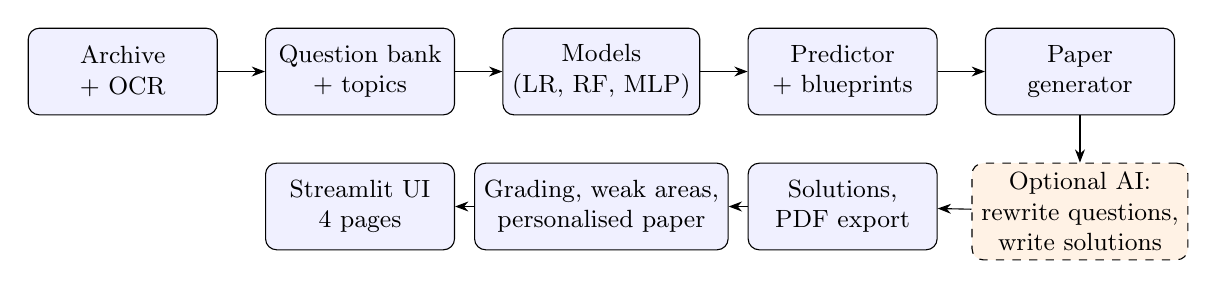
\begin{tikzpicture}[box/.style={draw,rounded corners,align=center,minimum height=1.1cm,minimum width=2.4cm,font=\small,fill=blue!6},
  ai/.style={draw,rounded corners,dashed,align=center,minimum height=1.1cm,minimum width=2.4cm,font=\small,fill=orange!10},
  >=Stealth,node distance=0.6cm]
\node[box] (a) {Archive\\+ OCR};
\node[box,right=of a] (b) {Question bank\\+ topics};
\node[box,right=of b] (c) {Models\\(LR, RF, MLP)};
\node[box,right=of c] (d) {Predictor\\+ blueprints};
\node[box,right=of d] (e) {Paper\\generator};
\node[ai,below=of e] (f) {Optional AI:\\rewrite questions,\\write solutions};
\node[box,below=of d] (g) {Solutions,\\PDF export};
\node[box,below=of c] (h) {Grading, weak areas,\\personalised paper};
\node[box,below=of b] (i) {Streamlit UI\\4 pages};
\draw[->] (a)--(b); \draw[->] (b)--(c); \draw[->] (c)--(d); \draw[->] (d)--(e);
\draw[->] (e)--(f); \draw[->] (f)--(g); \draw[->] (g)--(h); \draw[->] (h)--(i);
\end{tikzpicture}}
\caption{System overview. Dashed boxes need an API key; without one the application still works with real past questions and
archived solutions.}
\label{fig:system}
\end{figure}

\subsection{Browsing past papers}
The library layer lists all 130 subjects in the archive, groups papers into Final, Mid~1, Mid~2 and Quiz~$n$, and links every
paper to its real original file on GitHub (view and raw download), even when its text could not be read. Readable papers can
also be opened as questions.

\subsection{Prediction}
The predictor takes an exam of quiz, mid1, mid2 or final. Mid~1 and Mid~2 use the mid model and then re-weight each topic by how
often it appeared in earlier Mid~1 versus Mid~2 papers (shrunk toward the overall mid rate), only when at least three earlier
papers of that kind exist. Uploaded recent papers join the history for that prediction only, and topics already examined
earlier in the target year are flagged. Each topic gets a probability and a band (likely, possible, unlikely). Figure~\ref{fig:topics}
shows a real forecast.

\begin{figure}[!htb]
\centering
\maybefig{width=0.85\linewidth}{figures/fig_predicted_topics.png}
\caption{Topic forecast of the application for Artificial Intelligence, Final 2026 (logistic regression). The dashed line is
the decision threshold.}
\label{fig:topics}
\end{figure}

\subsection{Syllabus and uploaded papers}
A parser turns an outline or a pasted topic list into items and reads the \emph{MIDTERM EXAM 1/2} markers of real outlines to
suggest Mid~1 and Mid~2 scopes. A file reader handles text PDFs, scanned PDFs, Word, text and photographs. The word-based
syllabus matcher was evaluated on 29 real outlines: mean AUC 0.59 for separating a subject's own questions from other
subjects' questions, strong on clean outlines (about 0.82 for Theory of Automata and Software Design and Analysis) and weak
elsewhere. The syllabus is therefore a soft, visible signal: the student reviews and edits the parsed items, the generator uses
the match as a preference and shows it per question, and an optional strict mode filters.

\subsection{Predicted paper generator}
The generator builds a paper from real data. The structure (number of questions, total marks from the papers' stated totals,
question-type mix and difficulty mix) comes from the blueprint of real past papers of that exam kind. Topics come from the model,
with about 20\% of the questions reserved for less-predicted areas so that surprises are not missed. For each slot a real past
question is chosen to match the wanted type and difficulty, preferring recent questions and syllabus matches; near-duplicates are
avoided, cut-off or garbled questions (a fragment, scan damage, a missing question stem) are skipped, marks are scaled to the
typical total after capping noisy extremes, and the result is reproducible for the same inputs and seed. Each question carries
its reason, source (for example ``Mid 1 2024''), a one-to-five likelihood and a code-style flag, and the paper carries notes
that explain what was done. A default duration for the timer comes from the real papers of that kind. Table~\ref{tab:sample} lists
the structure of a generated paper.

\begin{table}[!htb]
\centering
\small
\begin{tabular}{clllll}
\toprule
No. & Topic keywords & Type & Difficulty & Likelihood & Source \\
\midrule
1 & uniform, cost search & other & easy & 2 & Final 2017 \\
2 & weights, regression & code & medium & 2 & Final 2020 \\
3 & heuristic, admissibility & other & medium & 1 & Mid 1 2022 \\
4 & search, path, nodes & numerical & hard & 5 & Mid 1 2026 \\
5 & fitness, chromosome & other & hard & 5 & Final 2016 \\
6 & game, pruning, minimax & numerical & hard & 4 & Mid 1 2026 \\
7 & decision tree, training & theory & hard & 4 & Final 2017 \\
\bottomrule
\end{tabular}
\caption{Structure of a generated paper (Artificial Intelligence, Final 2026): 7 questions, 55 marks, 180 minutes; one
question from a less-predicted area. Question texts are omitted here; see the application screenshots in Section~\ref{sec:ui}.}
\label{tab:sample}
\end{table}

An important design finding is that predicted questions are real past questions chosen for predicted topics, because exact
questions almost never repeat. Writing new questions needs a language model, which is added as an optional step
(Section~\ref{sec:llm}).

\subsection{Solutions and PDF export}
The archive holds solved copies of many papers. Pairing each question to the most similar chunk of its solved copy, together
with inline solutions, gives a real solution for roughly one question in eight (quality varies and notes say so). The
solution service tries the archive first, then an optional language model, caches AI solutions on disk, labels them
``AI-generated: verify'' and otherwise returns an honest ``none'' with the reason. A pure-Python PDF export covers the
``Download as PDF'' button, for the paper alone or with solutions.

%=====================================================================
\section{Language-Model Layer}
\label{sec:llm}

Language models are optional: the application is fully usable without a key, and every failure is turned into a readable
message instead of a crash.

\textbf{Client.} One small client speaks to several providers (Gemini, Groq, Mistral, Anthropic) over plain HTTPS. Keys are read
from environment variables or a local \texttt{.env} file and never stored in code. If the main provider fails (quota, busy server,
wrong model name) the client tries the next model of the same provider (each Gemini model has its own free quota) and then every
other provider whose key is set. Errors are shown in short plain language without raw server output.

\textbf{AI-written questions.} After a paper is generated, one batched call rewrites all its questions as new, similar
questions of the same topic, type and difficulty. Every rewritten question is checked (length, marks, no leftover numbering). If
the call fails or a question does not pass, that question stays the real past question, tidied by rule-based formatting.
Rule-based tidying runs without any AI: it strips page headers, watermarks (for example ``CamScanner''), term and campus
lines, and splits the text into lines for bullets, sub-parts and code comments.

\textbf{Solutions in the background.} Right after a paper is made, a background job fetches archived solutions at once and
asks the model for the missing ones in two parallel threads (to respect free-plan rate limits). The solution page shows a note
that the AI is writing a solution and fills it in by itself when it arrives; results are cached on disk, so repeats are
instant.

%=====================================================================
\section{Grading, Weak Areas and Personalisation}
\label{sec:feature5}

After attempting a paper (with the timer in exam mode) the student uploads photographs of their answers. A vision model
transcribes handwriting and compares it with the solution (archived or AI-written) to give a mark with a short reason per
question; the student can review and correct every mark, and unreadable or unmarked answers are excluded and listed. From the
marks the analysis computes the score per topic, difficulty and question type. A topic below 50\% is \emph{weak}, from 75\% it is
\emph{strong}; a weak area resting on a single question is labelled as a hint, not a fact. Attempts are saved on the student's
own computer only and are never uploaded.

The \textbf{personalised paper} reuses the generator with a tilt: weakness is estimated from the latest attempt (70\%) and the
last five attempts of the subject (30\%, newest counting most), up to six weak topics get about half of the main questions,
the rest still follow the prediction, the less-predicted questions stay, and the questions of the paper just attempted are
excluded so that the student gets new ones.

%=====================================================================
\section{User Interface}
\label{sec:ui}

The interface is a Streamlit~\cite{streamlit} multi-page application with a neo-brutalist theme (sage background, cream cards, lime and red
accents, tilted sticky notes and stamps). It has four pages: \textbf{Home}, \textbf{Past papers}, \textbf{Upcoming paper} and
\textbf{My results}. On the Upcoming paper page the student chooses a subject and an exam, optionally uploads recent papers
and a syllabus (shown as editable chips) and sets the number of questions and total marks. The result opens as a
``declassified'' predicted paper with a likelihood stamp per question, a ``How this paper was made'' panel in plain sentences, a
timer with a default duration taken from real papers, an exam mode, a solved paper and a PDF download. My results holds the
upload of answers, review and marking, weak-area report, history and the personalised paper. Figures~\ref{fig:ui1}
to~\ref{fig:ui3} show the pages.

\begin{figure}[!htb]
\centering
\maybefig{width=0.48\linewidth}{figures/ui_home.png}\hfill
\maybefig{width=0.48\linewidth}{figures/ui_past_papers.png}
\caption{Home page (left) and the Past papers page of a subject (right).}
\label{fig:ui1}
\end{figure}

\begin{figure}[!htb]
\centering
\maybefig{width=0.48\linewidth}{figures/ui_upcoming_form.png}\hfill
\maybefig{width=0.48\linewidth}{figures/ui_predicted_paper.png}
\caption{Upcoming paper: the request form (left) and the predicted paper with likelihood stamps (right).}
\label{fig:ui2}
\end{figure}

\begin{figure}[!htb]
\centering
\maybefig{width=0.48\linewidth}{figures/ui_solved.png}\hfill
\maybefig{width=0.48\linewidth}{figures/ui_my_results.png}
\caption{The solved paper (left) and the My results page with weak areas (right).}
\label{fig:ui3}
\end{figure}

\begin{figure}[!htb]
\centering
\maybefig{width=0.48\linewidth}{figures/ui_exam_mode.png}\hfill
\maybefig{width=0.48\linewidth}{figures/ui_personalised.png}
\caption{Exam mode with the timer (left) and a personalised paper (right).}
\label{fig:ui4}
\end{figure}

%=====================================================================
\section{Testing and Engineering Practice}
\label{sec:testing}

The repository has more than 200 automated tests (pytest) that run without a network or an API key. They cover: the serving
features equalling the training features on every row of train, validation and test; the saved topic models reproducing the
stored topic ids; no leakage when only target-year papers change; the metrics and bootstrap; the question segmenter, marks
parser and quality filter; the syllabus parser; the generator (structure, determinism, no near-duplicates); the solution
service and background jobs with a fake model; the language-model client with mocked HTTP (retries, fallback chain, readable
errors); grading, analysis and the personalised paper; and every Streamlit page with the Streamlit testing framework. A full
rebuild of the data and models runs with one command (\texttt{scripts/rebuild\_all.py}). Large artefacts (trained models, the
question bank derived from exam papers) are shipped as a runtime bundle fetched by a script and are not stored in Git.

%=====================================================================
\section{Limitations}
\label{sec:limits}
\begin{itemize}
\item \textbf{Predicted questions are mostly real past questions.} Probabilities and likelihood squares are rankings that are
over-estimated; AI-rewritten questions need a key and a human check; difficulty is a proxy.
\item \textbf{Not statistically separated from rules.} The learned models lead the best rule by 0.014 to 0.035 AUC, within
the intervals. No cold-start (never-seen topic) evidence exists in the test split.
\item Topic clusters are keyword clusters, not syllabus topics (median silhouette 0.093); some capture generic wording.
\item Marks parse for about half of the questions; about 20\% of types are ``other''; question-type accuracy has not been
measured against hand labels.
\item 349 clean papers remain unreadable (mostly handwritten); the exam-rule filter loses about one borderline chunk in twelve.
\item Only 37 subjects are supported because topics are fitted on years up to 2022 for honest evaluation.
\item Archived solutions can be partial and an inspected pairing was misaligned; AI solutions must be checked by the student.
\item Free language-model plans have rate and daily limits, so AI steps can be slow or fall back to real questions.
\item Photo grading by a vision model can misread handwriting; every mark is reviewable by the student.
\item The generator has not yet been scored paper by paper against real exams (topic coverage of a predicted paper versus the
real paper); only the topic-level models are evaluated quantitatively.
\item No instructor information is used. The tool is a study aid and is not guaranteed to match any exam.
\end{itemize}

%=====================================================================
\section{Future Work}
\label{sec:future}
\begin{enumerate}
\item A paired bootstrap of model versus rule, and a paper-level backtest of the generator (how many topics of the real exam
it covers, against simple baselines).
\item Production mode: fit topics and models on all years so newer courses are supported.
\item Add-your-own-subject for unsupported subjects, and an OCR rescue pass for papers that a vision model could read.
\item Hand-labelling a sample of question types and difficulty to quote a measured accuracy.
\item Semantic (embedding) matching for syllabus items and topics, richer question-level features for the models, and a study of
cold-start topics once the data contain them.
\item Public deployment of the Streamlit application.
\end{enumerate}

%=====================================================================
\section{Conclusion}
\label{sec:concl}
SpillThePaper shows that an archive of unstructured past papers can be turned into a working study tool. The data work
(cleaning, OCR, question bank) mattered as much as the modelling: removing exam rules and headers and recovering scanned papers
raised the number of supported subjects from 28 to 37 and doubled the test set. A time-based, leakage-safe evaluation shows
that learned models reach a test AUC-ROC of 0.850 to 0.871, slightly ahead of simple history rules and clearly more precise than
the rule ``appeared five times'', but not statistically separated from the best rule. The application turns the forecast into a
predicted paper with a realistic structure and timer, solutions that are written in the background, photo-based grading,
weak-area analysis and a personalised follow-up paper, while keeping the real, tidied past questions as the fallback whenever
AI is unavailable.

%=====================================================================
\section{Reproducibility and Repository}
\label{sec:repro}
The code is at \url{https://github.com/Minahilbasalat/SpillThePaper}. Trained model weights and the runtime bundle are hosted
at \url{\weightsurl}. To run the application: create a virtual environment, \texttt{pip install -r requirements.txt}, fetch the
runtime bundle with \texttt{python scripts/get\_runtime.py}, run \texttt{python -m pytest tests -q}, then
\texttt{streamlit run app/Home.py}. An optional language-model key is placed in a local \texttt{.env} file
(\texttt{GEMINI\_API\_KEY=...}; \texttt{GROQ\_API\_KEY=...} adds a fallback provider). To rebuild the data and models use
\texttt{python scripts/rebuild\_all.py}. Key folders: \texttt{data scripts/} (collection and preprocessing), \texttt{src/data/}
(OCR, segmentation, cleaning, question features, topics), \texttt{src/models/} and \texttt{src/evaluation/} (training and
evaluation), \texttt{src/inference/} (the backend), \texttt{app/} (the interface), \texttt{results/} (metrics),
\texttt{report/} (this report) and \texttt{tests/}.

%=====================================================================
\begin{thebibliography}{99}\small
\bibitem{atm} S.~Muzammil et al., \emph{Academic-Time-Machine}: a student-maintained archive of FAST-NUCES past papers, GitHub repository, \url{https://github.com/saleha-muzammil/Academic-Time-Machine} (pinned commit e0e1975).
\bibitem{sklearn} F.~Pedregosa et al., ``Scikit-learn: Machine learning in Python,'' \emph{Journal of Machine Learning Research}, vol.~12, pp.~2825--2830, 2011.
\bibitem{pytorch} A.~Paszke et al., ``PyTorch: An imperative style, high-performance deep learning library,'' in \emph{Advances in Neural Information Processing Systems 32}, 2019.
\bibitem{adam} D.~P. Kingma and J.~Ba, ``Adam: A method for stochastic optimization,'' in \emph{International Conference on Learning Representations (ICLR)}, 2015.
\bibitem{rf} L.~Breiman, ``Random forests,'' \emph{Machine Learning}, vol.~45, no.~1, pp.~5--32, 2001.
\bibitem{tfidf} G.~Salton and C.~Buckley, ``Term-weighting approaches in automatic text retrieval,'' \emph{Information Processing \& Management}, vol.~24, no.~5, pp.~513--523, 1988.
\bibitem{kmeans} S.~P. Lloyd, ``Least squares quantization in PCM,'' \emph{IEEE Transactions on Information Theory}, vol.~28, no.~2, pp.~129--137, 1982.
\bibitem{silhouette} P.~J. Rousseeuw, ``Silhouettes: A graphical aid to the interpretation and validation of cluster analysis,'' \emph{Journal of Computational and Applied Mathematics}, vol.~20, pp.~53--65, 1987.
\bibitem{bootstrap} B.~Efron, ``Bootstrap methods: Another look at the jackknife,'' \emph{The Annals of Statistics}, vol.~7, no.~1, pp.~1--26, 1979.
\bibitem{brier} G.~W. Brier, ``Verification of forecasts expressed in terms of probability,'' \emph{Monthly Weather Review}, vol.~78, no.~1, pp.~1--3, 1950.
\bibitem{tesseract} R.~Smith, ``An overview of the Tesseract OCR engine,'' in \emph{Proc. Ninth International Conference on Document Analysis and Recognition (ICDAR)}, vol.~2, pp.~629--633, 2007.
\bibitem{pymupdf} Artifex Software, \emph{PyMuPDF} documentation, \url{https://pymupdf.readthedocs.io}.
\bibitem{streamlit} Streamlit Inc., \emph{Streamlit} documentation, \url{https://docs.streamlit.io}.
\end{thebibliography}

\end{document}
